%!TEX TS-program = xelatex
%!TEX options = -aux-directory=Debug -shell-escape -file-line-error -interaction=nonstopmode -halt-on-error -synctex=1 "%DOC%"
\documentclass{article}
\input{LaTeX-Submodule/template.tex}

% Additional packages & macros
\setminted{linenos,frame=lines}

% Header and footer
\newcommand{\unitName}{Embedded Systems}
\newcommand{\unitTime}{Semester 1, 2025}
\newcommand{\unitCoordinator}{Dr Chris Lehnert}
\newcommand{\documentAuthors}{Tarang Janawalkar}

\fancyhead[L]{\unitName}
\fancyhead[R]{\leftmark}
\fancyfoot[C]{\thepage}

% Copyright
\usepackage[
    type={CC},
    modifier={by-nc-sa},
    version={4.0},
    imagewidth={5em},
    hyphenation={raggedright}
]{doclicense}

\date{}

\begin{document}
%
\begin{titlepage}
    \vspace*{\fill}
    \begin{center}
        \LARGE{\textbf{\unitName}} \\[0.1in]
        \normalsize{\unitTime} \\[0.2in]
        \normalsize\textit{\unitCoordinator} \\[0.2in]
        \documentAuthors
    \end{center}
    \vspace*{\fill}
    \doclicenseThis
    \thispagestyle{empty}
\end{titlepage}
\newpage
%
\tableofcontents
\newpage
%
\section{Introduction}
\subsection{Definition of an Embedded System}
An embedded system is a combination of computer hardware and software
designed for a specific function or functions within a larger system.
These systems typically contain computer hardware \textit{within} their
implementation and are used in devices to simplify system design and
provide flexibility. Often, the user is unaware that a processor is
present in the device as an embedded system comprises a suite of
different components that communicate with each other to perform a
specific task. These components include the processor, memory, and
analog/digital ports---which form the microcontroller---and ports that
are connected to various input/output devices such as sensors,
actuators, and user interfaces---each of which interact with the
environment. This is illustrated in the figure below, where the grey
box represents the embedded system.
\begin{figure}[H]
    \centering
    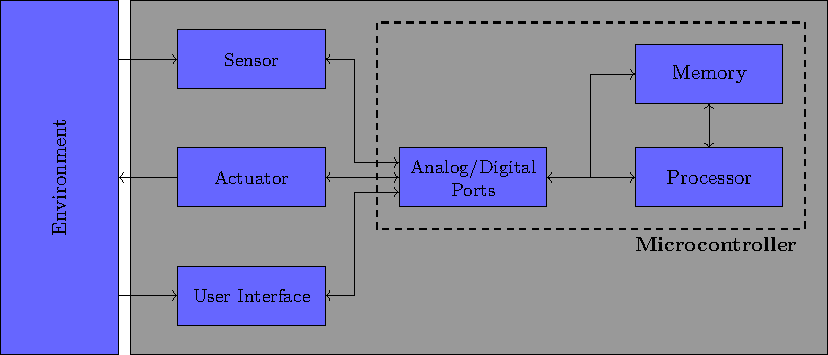
\includegraphics[width = \linewidth]{figures/embedded_system_structure.pdf}
    % \caption{} % \label{}
\end{figure}
\subsubsection{Types of Embedded Systems}
Embedded systems can be classified into three main categories:
\begin{itemize}
    \item \textbf{Centralised:} One node performs all work.
    \item \textbf{Distributed:} Nodes distribute work across sub-nodes.
    \item \textbf{Decentralised:} Nodes are only connected to peers in a network.
\end{itemize}
\subsection{Advanced RISC Machines}
Advanced RISC Machine (ARM) is a family of Instruction Set
Architectures (ISAs) for computer processors. These ISAs are developed
and designed by Arm Holdings so that they can be licensed to other
companies that design their own ARM-based processors. ARM processors
are found in many battery operated devices such as mobile phones,
tablets, embedded systems, and some newer laptops.

Reduced Instruction Set Computer (RISC) processors are popular in such
applications due to their high performance per watt and ability to
execute all instructions in a single cycle. Additionally, because the
architecture uses fixed-length instructions, instructions are also
easier to pipeline, leading to increased parallelism. The RISC
architecture focuses on small and highly-optimised instructions rather
than the highly-specialised set of instructions found on Complex
Instruction Set Computer (CISC) architectures such as x86. Although
this may seem restrictive, this allows instructions to be executed at a
greater frequency resulting in improved performance. Complex operations
can then be performed in software using these instructions.
\subsubsection{ARM Cortex Cores}
ARM develops many families of processing cores for a range of different
functions:
\begin{itemize}
    \item \textbf{Cortex-A}: Highest performance cores---optimised for rich operating systems.
    \item \textbf{Cortex-R}: Fast response cores---optimised for high-performance, hard real-time applications.
    \item \textbf{Cortex-M}: High efficiency cores---optimised for discrete processing and microcontrollers.
    \item \textbf{SecurCore}: Tamper resistant cores---optimised for security applications.
\end{itemize}
\subsection{Characteristics of an Embedded System}
Embedded systems are characterised by several features. At a high
level, they may be designed to be:
\begin{itemize}
    \item Highly stable
    \item Time specific
    \item Task specific
    \item Cost effective
    \item Minimal in interface
    \item Easy to operate
    \item Real-time
    \item High-efficiency
    \item Reliable
    \item Memory constrained
    \item Power constrained
    \item Fault tolerant
\end{itemize}
\subsubsection{Design Goals}
These characteristics lead to several design goals in embedded systems
such as:
\begin{itemize}
    \item Reliability: Some systems may be critical to a mission, or
          life-threatening, and must be able to operate 24/7 without
          rebooting.
    \item Performance: Systems may need to respond to many events
          within a time frame using resources such as computing speed
          and power effectively. Constraints may need to be placed on
          inputs to prevent buffer overflows, and inaccuracies from
          floating-point calculations must be properly handled.
    \item Cost: Systems may be marketed to consumers and must therefore
          manufacturing minimise cost and be easy to produce.
\end{itemize}
\subsection{Real-Time Applications}
A system is said to be real-time if the total correctness of an
operation not only depends on its logical correctness, but also upon
the time in which it is performed. A primary design goal of real-time
systems is \textbf{meeting deadlines}.
\begin{itemize}
    \item \textbf{Soft real-time systems} execute as fast as possible requiring
          on explicit deadline on the response time.
    \item \textbf{Hard real-time systems} impose a strict deadline on the
          response time. If the deadline is missed, the system fails.
\end{itemize}
\subsubsection{Real-Time Operating Systems}
Embedded systems are typically developed using low-level programming
languages such as C, C++, and assembly, for their performance and
reliable compilation. The compilation process is different from that of
a desktop application where code is compiled into an executable file
which can be executed by the operating system. Instead, embedded
systems (or those with sufficient resources) make use of
\textbf{real-time kernel} libraries alongside application code to
produce a single binary image that is flashed onto the device. These
systems are known as real-time operating systems (RTOS). The kernel is
software that manages this real-time system by providing abstractions
for creating threads (tasks), scheduling, input/output operations,
memory management, and other functions in an operating system.
\subsection{Tiva C Series Microcontrollers}
This unit uses the Texas Instruments Tiva C series TM4C1294NCPDT
microcontroller which is housed on the EK-TM4C1294XL evaluation board.
This microcontroller chip is based on an ARM Cortex-M4 core and
includes several on-chip peripherals such as an Ethernet controller,
USB interface, analog-to-digital converters (ADCs), and timers. The
evaluation board also provides additional hardware such as LEDs,
switches, a touch screen, and other input/output devices, all of which
can be interfaced with the microcontroller.
\subsubsection{Arm Cortex-M4 Processor}
Some technical specifications of the Cortex-M4 processor are described
below:
\begin{itemize}
    \item \textbf{Architecture}: Armv7E-M
    \item \textbf{Bus Interface}: 3x Advanced Microcontroller Bus Architecture 3 Advanced High-performance Bus-Lite (AHBA 3 AHB-Lite) interface (Harvard bus architecture)
    \item \textbf{Instruction Set Architecture Support}: Thumb or Thumb-2\footnote{The
              thumb instruction set is a subset of the most commonly used 32-bit ARM
              instructions. Thumb instructions are 16 bits long and have
              corresponding 32-bit ARM instructions that perform the same
              function. They are used to reduce code size and improve
              performance in memory-constrained applications. Thumb2 provides
              enhancements to Thumb by introducing a new conditional instruction
              amongst other improvements.}, hardware divide, single-cycle multiply, etc.
    \item \textbf{Pipeline}: 3-stage (Fetch-Decode-Execute)
\end{itemize}
A block diagram of the Cortex-M4 processor, and its register set are
shown below.
\begin{figure}[H]
    \centering
    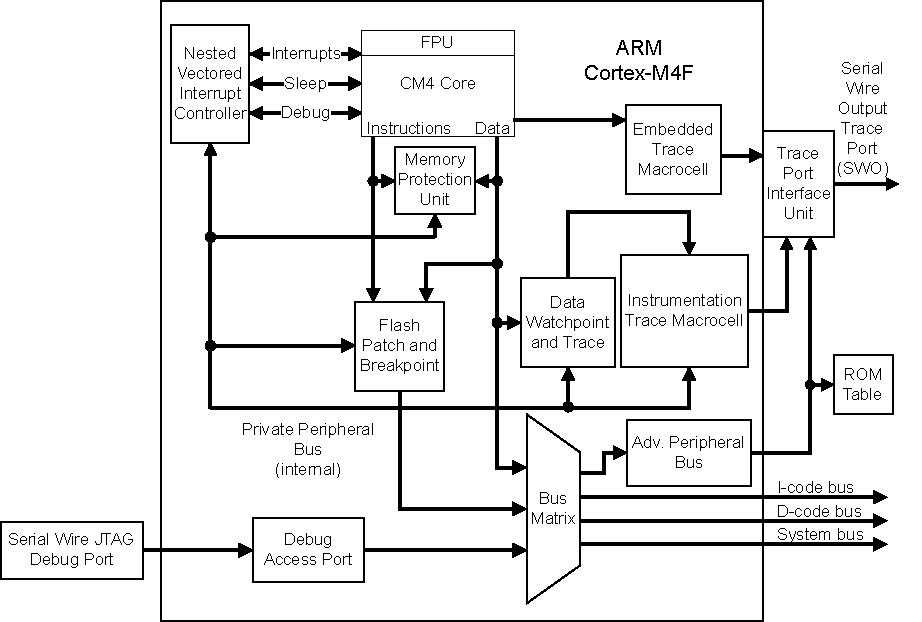
\includegraphics[width = \linewidth]{figures/cortex_m4_block_diagram.pdf}
    \caption{Block diagram of the Cortex-M4 processor.}
\end{figure}
\begin{figure}[H]
    \centering
    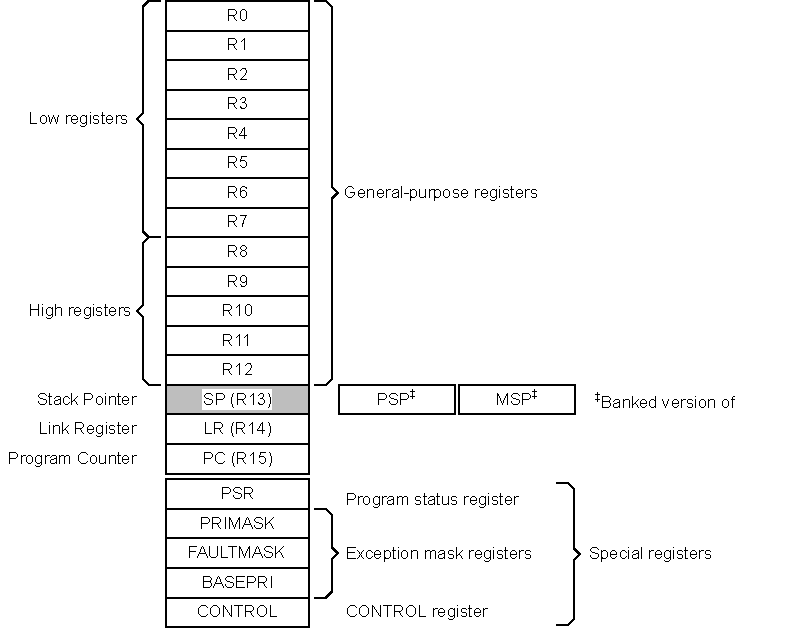
\includegraphics[width = \linewidth]{figures/cortex_m4_register_set.pdf}
    \caption{Register set of the Cortex-M4 processor.}
\end{figure}
\subsubsection{Programming Models}
Tiva C series microcontrollers can be programmed using the
\textbf{Direct Register Access Model} where the application accesses
hardware registers directly using pointers and bitwise operations. This
model results in small and more efficient code.

The registers in this model can be accessed by including the
\texttt{tm4c1294ncpdt.h} header file, which contains register
definitions for all peripherals on the Tiva C series microcontroller.
\begin{minted}{c}
#include "inc/tm4c1294ncpdt.h"
\end{minted}
The macros in this header file use the following naming conventions:
\begin{itemize}
    \item \textbf{Suffixes}:
          \begin{itemize}
              \item \mintinline{c}{_R}: Access to the memory mapped register.
              \item \mintinline{c}{_M}: Mask for a multi-bit field.
              \item \mintinline{c}{_S}: Shift value for field alignment.
          \end{itemize}
    \item \textbf{Register Name Structure}: \mintinline{c}{<MODULE><INSTANCE>_<REGISTER>_R}
    \item \textbf{Bit Field Name Structure}: \mintinline{c}{<MODULE><INSTANCE>_<REGISTER>_<FIELD>}. Bit fields
          with multiple values are often suffixed with \mintinline{c}{_M}, \mintinline{c}{_S}, or a value.
\end{itemize}
Alternatively, we can use the \textbf{Software Driver Model} where the
application uses a development API such as the \textbf{TivaWare}
software development kit (SDK) to access hardware registers. This model
aims to simplify the development process by providing functions for
accessing peripherals such as GPIO, UART, I2C, SPI, and ADC.
\subsection{Microcontroller Architecture}
A microcontroller is made up of a microprocessor, memory, peripherals,
and I/O. Communication between the microprocessor and these devices is
facilitated through the system bus that consists of an address bus,
data bus, and control bus\footnote{A bus refers to a group of lines
carrying digital signals.}. This bus allows shared communication
between a single processor and device at a time. To overcome this
limitation and allow multiple devices to communicate with multiple
processors concurrently, a bus matrix is often used instead of, or in
addition to, the system bus. Furthermore, microprocessor architecture
also determines whether code memory and data memory are accessed via
the same data bus, where:
\begin{itemize}
    \item \textbf{von Neumann Bus Architecture} accesses code and data memory from the same bus.
    \item \textbf{Harvard Bus Architecture} accesses code and data memory from two separate buses, called the instruction code bus (I-code bus) and the data code bus (D-code bus).
\end{itemize}
\subsection{Microcontroller Memory}
The TM4C1294NCPDT microcontroller is integrated with the following set
of on-chip memory:
\begin{itemize}
    \item \textbf{Non-Volatile Memory} (retains data when powered off):
          \begin{itemize}
              \item \qty{1024}{K.B} \textbf{Flash Memory} (\(4 \times \qty{256}{K.B}\) banks) used for storing program code.
              \item \qty{6}{K.B} \textbf{Electronically Erasable Programmable Read-Only Memory (EEPROM)} used for storing non-volatile data.
              \item \textbf{Internal Read-Only Memory (ROM)} loaded with
                    TivaWare for C Series software: TivaWare Peripheral
                    Driver Library and TivaWare Boot Loader.
          \end{itemize}
    \item \textbf{Volatile Memory} (loses data when powered off):
          \begin{itemize}
              \item \qty{256}{K.B} \textbf{Single-Cycle Static Random Access Memory (SRAM)} used for very fast data access and frequent
                    read/write operations. This memory is the runtime memory for the
                    program stack, peripheral registers, and runtime variables.
          \end{itemize}
\end{itemize}
\subsubsection{Memory Map}
Desktop architectures typically have separate address spaces for memory
and peripherals, where input and output devices are mapped to a
separate address space. However, the TM4C1294NCPDT microcontroller uses
a shared address space for memory and peripherals, which is known as
the \textbf{memory map}.
\begin{table}[H]
    \centering
    \begin{tabular}{llp{5cm}}
        \toprule
        \textbf{Address Range}                       & \textbf{Memory Region} & \textbf{Description}                                                                                                      \\
        \midrule
        \mintinline{rust}{0x0000_0000 - 0x1FFF_FFFF} & Code                   & This executable region is for program code. Data can also be stored here.                                                 \\
        \mintinline{rust}{0x2000_0000 - 0x3FFF_FFFF} & SRAM                   & This executable region is for data. Code can also be stored here. This region includes bit band and bit band alias areas. \\
        \mintinline{rust}{0x4000_0000 - 0x5FFF_FFFF} & Peripheral             & This region includes bit band and bit band alias areas.                                                                   \\
        \mintinline{rust}{0x6000_0000 - 0x9FFF_FFFF} & External RAM           & This executable region is for data.                                                                                       \\
        \mintinline{rust}{0xA000_0000 - 0xDFFF_FFFF} & External device        & This region is for external device memory.                                                                                \\
        \mintinline{rust}{0xE000_0000 - 0xE00F_FFFF} & Private peripheral bus & This region includes the NVIC, system timer, and system control block.                                                    \\
        \mintinline{rust}{0xE010_0000 - 0xFFFF_FFFF} & Reserved               & -                                                                                                                         \\
        \bottomrule
    \end{tabular}
    \caption{Memory Access Map on the TM4C1294NCPDT Microcontroller.}
\end{table}
\subsubsection{Bit-Banding}
The ARM Cortex-M4 processor supports a feature called
\textbf{bit-banding} which maps a full word of memory to a single bit
in the bit-band region. This eliminates the need for read-modify-write
operations, as individual bits can be set, cleared, or toggled directly
from an alias address. This technique is used on the TM4C1294NCPDT as
it uses a 32-bit word size, resulting in \qty{4}{G.B} of addressable
memory, of which, peripherals only use a small portion. The remaining
region of memory is therefore used for alias addresses that serve this
purpose.
\section{Microcontroller Peripherals}
The following sections highlight the functionality of various
peripherals and provide examples of their configuration using the
TivaWare Peripheral Driver Library. All information in this section is
taken from the User's Guide document.
\subsection{System Control}
System control determines the overall operation of the device by:
\begin{itemize}
    \item controlling the system clock,
    \item configuring which peripherals are enabled,
    \item configuring the device and its resets, and by
    \item providing information about the device.
\end{itemize}
\subsubsection{System Clock}
The main system clock is used to clock the processor and all
peripherals on the device. The system clock frequency is determined
through the following steps:
\begin{enumerate}
    \item \textbf{Select the input source:}

          Choose an oscillator source (internal oscillator or external
          crystal) and configure the frequency of the oscillator.
    \item \textbf{Apply a frequency multiplier:} (optional)

          A Phase-Locked Loop (PLL) can be used to multiply an input
          frequency using a Voltage Controlled Oscillator (VCO).
    \item \textbf{Apply Frequency Divider:} (optional)

          The system clock divider can be used to divide the output
          frequency of the PLL or oscillator source.
    \item \textbf{Select the system clock source:}

          Choose whether the system clock is driven by the PLL output
          or directly by the oscillator source.
\end{enumerate}

\medskip
\textbf{Oscillator Source}

The oscillator source can be one of the following:
\begin{itemize}
    \item \mintinline{c}{SYSCTL_OSC_MAIN} to use an external crystal or oscillator.
    \item \mintinline{c}{SYSCTL_OSC_INT} to use the \qty{16}{M.Hz} precision internal oscillator.
    \item \mintinline{c}{SYSCTL_OSC_INT30} to use the internal low frequency oscillator.
    \item \mintinline{c}{SYSCTL_OSC_EXT32} to use the hibernate modules \qty{32.786}{k.Hz} oscillator.
\end{itemize}
When using an external crystal, the frequency is set using the
macro \mintinline{c}{SYSCTL_XTAL_<frequency>MHZ} where
\mintinline{c}{<frequency>} is the frequency of the crystal in \unit{M.Hz}.

\medskip
\textbf{System Clock Source}

The system clock source may be configured to use the output of the PLL
or be directly driven by the oscillator source using one of the
following macros:
\begin{itemize}
    \item \mintinline{c}{SYSCTL_USE_PLL} is used to select the PLL output as the system clock.
    \item \mintinline{c}{SYSCTL_USE_OSC} is used to choose one of the oscillators as the system clock.
\end{itemize}
When using the PLL, the VCO frequency can be configured using one of the
following macros:
\begin{itemize}
    \item \mintinline{c}{SYSCTL_CFG_VCO_480} to set the PLL VCO output to \qty{480}{M.Hz}
    \item \mintinline{c}{SYSCTL_CFG_VCO_320} to set the PLL VCO output to \qty{320}{M.Hz}
\end{itemize}
The \mintinline{c}{SysCtlClockFreqSet()} function attempts to match the
requested system clock frequency to the closest possible value based on
the configuration of the device clocking.
\subsubsection{SysCtlClockFreqSet()}
\textbf{Prototype:}
\begin{minted}{c}
uint32_t SysCtlClockFreqSet(uint32_t ui32Config, uint32_t ui32SysClock);
\end{minted}
\textbf{Parameters:}
\begin{itemize}
    \item \mintinline{c}{ui32Config} is the required configuration of the device clocking.
    \item \mintinline{c}{ui32SysClock} is the requested processor frequency.
\end{itemize}
\textbf{Returns:}
\medskip

The actual configured system clock frequency in Hz or zero if the value
could not be changed due to a parameter error or PLL lock failure.

\medskip
\textbf{Example:}
\begin{minted}{c}
#include "inc/tm4c1294ncpdt.h"

int main(void) {
    // Use a 25 MHz external crystal oscillator with a PLL VCO output of
    // 480 MHz.
    // The desired system clock frequency is 120 MHz which will require
    // a system clock divider of 4.
    SysCtlClockFreqSet(SYSCTL_XTAL_25MHZ | SYSCTL_OSC_MAIN |
                       SYSCTL_USE_PLL | SYSCTL_CFG_VCO_480, 120000000);

    // ...
}
\end{minted}
\subsubsection{Peripheral Enable}
Most peripherals are disabled by default to reduce power consumption. A
peripheral can be enabled using the system control module.

\medskip
\textbf{SysCtlPeripheralEnable()}

\textbf{Prototype:}
\begin{minted}{c}
void SysCtlPeripheralEnable(uint32_t ui32Peripheral)
\end{minted}
\textbf{Parameters:}
\begin{itemize}
    \item \mintinline{c}{ui32Peripheral} is the peripheral to enable.
\end{itemize}
\textbf{Returns:}
\medskip
None.

\medskip
\textbf{Example:}
\begin{minted}{c}
#include "inc/tm4c1294ncpdt.h"

int main(void) {
    // Enable the GPIO Port A peripheral.
    SysCtlPeripheralEnable(SYSCTL_PERIPH_GPIOA);

    // ...
}
\end{minted}
\subsection{General Purpose Input/Output (GPIO)}
The General Purpose Input/Output (GPIO) module provides control over
GPIO ports and pins on the device. Each pin has the following
capabilities:
\begin{itemize}
    \item Can be configured as an input or an output. On reset, GPIOs
          default to being inputs.
    \item In input mode, can generate interrupts on high level, low
          level, rising edge, falling edge, or both edges.
    \item In output mode, can be configured for \qty{2}{m.A},
          \qty{4}{m.A}, or \qty{8}{m.A} drive strength. The
          \qty{8}{m.A} drive strength configuration has optional slew
          rate control to limit the rise and fall times of the signal.

          On reset, GPIOs default to \qty{2}{m.A} drive strength.
    \item Optional weak pull-up or pull-down resistors. On reset, GPIOs
          default to no pull-up or pulldown resistors.
    \item Optional open-drain operation. On reset, GPIOs default to
          standard push/pull operation.
    \item Can be configured to be a GPIO or a peripheral pin. On reset,
          the default is GPIO. Note that not all pins on all parts have
          peripheral functions, in which case the pin is only useful as
          a GPIO.
\end{itemize}
\subsubsection{GPIO Function API}
The GPIO API is broken into three groups of functions:
\begin{itemize}
    \item The GPIO pins are configured with
          \mintinline{c}{GPIODirModeSet()},
          \mintinline{c}{GPIOPadConfigSet()}, and
          \mintinline{c}{GPIOPinConfigure()}. The configuration can be
          read back with \mintinline{c}{GPIODirModeGet()} and
          \mintinline{c}{GPIOPadConfigGet()}.
    \item The GPIO pin state is accessed with
          \mintinline{c}{GPIOPinRead()} and
          \mintinline{c}{GPIOPinWrite()}.
    \item The GPIO interrupts are handled with
          \mintinline{c}{GPIOIntTypeSet()},
          \mintinline{c}{GPIOIntTypeGet()},
          \mintinline{c}{GPIOIntEnable()},
          \mintinline{c}{GPIOIntDisable()},
          \mintinline{c}{GPIOIntStatus()},
          \mintinline{c}{GPIOIntClear()},
          \mintinline{c}{GPIOIntRegister()}, and
          \mintinline{c}{GPIOIntUnregister()}.
\end{itemize}
\subsubsection{GPIO Peripheral Functions}
Many GPIO pins have other peripheral functions that can also use the
GPIO pins for peripheral pins. Several convenience functions are
provided to configure the pins in the required or recommended
input/output configuration. These functions are:
\begin{itemize}
    \item \mintinline{c}{GPIOPinTypeADC()}
    \item \mintinline{c}{GPIOPinTypeCAN()}
    \item \mintinline{c}{GPIOPinTypeComparator()}
    \item \mintinline{c}{GPIOPinTypeEPI()}
    \item \mintinline{c}{GPIOPinTypeEthernetLED()}
    \item \mintinline{c}{GPIOPinTypeEthernetMII()}
    \item \mintinline{c}{GPIOPinTypeGPIOInput()}
    \item \mintinline{c}{GPIOPinTypeGPIOOutput()}
    \item \mintinline{c}{GPIOPinTypeGPIOOutputOD()}
    \item \mintinline{c}{GPIOPinTypeI2C()}
    \item \mintinline{c}{GPIOPinTypeI2CSCL()}
    \item \mintinline{c}{GPIOPinTypeLCD()}
    \item \mintinline{c}{GPIOPinTypePWM()}
    \item \mintinline{c}{GPIOPinTypeQEI()}
    \item \mintinline{c}{GPIOPinTypeSSI()}
    \item \mintinline{c}{GPIOPinTypeTimer()}
    \item \mintinline{c}{GPIOPinTypeUART()}
    \item \mintinline{c}{GPIOPinTypeUSBAnalog()}
    \item \mintinline{c}{GPIOPinTypeUSBDigital()}
    \item \mintinline{c}{GPIOPinTypeWakeHigh()}
    \item \mintinline{c}{GPIOPinTypeWakeLow()}
    \item \mintinline{c}{GPIOPinWakeStatus()}
    \item \mintinline{c}{GPIODMATriggerEnable()}
    \item \mintinline{c}{GPIODMATriggerDisable()}
    \item \mintinline{c}{GPIOADCTriggerEnable()}
    \item \mintinline{c}{GPIOADCTriggerDisable()}
\end{itemize}
\subsection{General Purpose Timers}
The timer module provides two half-width timers/counters that can be
configured to operate independently as timers or event counters or to
operate as a combined full-width timer or Real Time Clock (RTC). Some
timers provide 16-bit half-width timers and a 32-bit full-width timer,
while others provide 32-bit half-width timers and a 64-bit full-width
timer. Two half-width timers provided by a timer module are referred to
as TimerA and TimerB, and the full-width timer is referred to as
TimerA.
\subsubsection{One-Shot \& Continuous Mode}
When configured as either a full-width or half-width timer, a timer can
be set up to run as a one-shot timer or a continuous timer. If
configured in one-shot mode, the timer ceases counting when it reaches
zero when counting down or the load value when counting up. If
configured in continuous mode, the timer counts to zero (counting down)
or the load value (counting up), then reloads and continues counting.
When configured as a full-width timer, the timer can also be configured
to operate as an RTC. In this mode, the timer expects to be driven by a
\qty{32.768}{K.Hz} external clock, which is divided down to produce 1
second clock ticks.
\subsubsection{Event Capture \& Pulse Width Modulation}
When in half-width mode, the timer can also be configured for event
capture or as a Pulse Width Modulation (PWM) generator. When configured
for event capture, the timer acts as a counter. It can be configured to
either count the time between events or the events themselves. The type
of event being counted can be configured as a positive edge, a negative
edge, or both edges. When a timer is configured as a PWM generator, the
input signal used to capture events becomes an output signal, and the
timer drives an edge-aligned pulse onto that signal.
\subsubsection{General Purpose Timer Function API}
The timer API is broken into three groups of functions:
\begin{itemize}
    \item Timer configuration is handled by
          \mintinline{c}{TimerConfigure()}, which performs the high
          level setup of the timer module; that is, it is used to set
          up full- or half-width modes, and to select between PWM,
          capture, and timer operations. Timer control is performed by
          \mintinline{c}{TimerEnable()},
          \mintinline{c}{TimerDisable()},
          \mintinline{c}{TimerControlLevel()},
          \mintinline{c}{TimerControlTrigger()},
          \mintinline{c}{TimerControlEvent()},
          \mintinline{c}{TimerControlStall()},
          \mintinline{c}{TimerRTCEnable()}, and
          \mintinline{c}{TimerRTCDisable()}.
    \item Timer content is managed with \mintinline{c}{TimerLoadSet()},
          \mintinline{c}{TimerLoadGet()},
          \mintinline{c}{TimerLoadSet64()},
          \mintinline{c}{TimerLoadGet64()},
          \mintinline{c}{TimerPrescaleSet()},
          \mintinline{c}{TimerPrescaleGet()},
          \mintinline{c}{TimerMatchSet()},
          \mintinline{c}{TimerMatchGet()},
          \mintinline{c}{TimerMatchSet64()},
          \mintinline{c}{TimerMatchGet64()},
          \mintinline{c}{TimerPrescaleMatchSet()},
          \mintinline{c}{TimerPrescaleMatchGet()},
          \mintinline{c}{TimerValueGet()},
          \mintinline{c}{TimerValueGet64()}, and
          \mintinline{c}{TimerSynchronize()}.
    \item The interrupt handler for the Timer interrupt is managed with
          \mintinline{c}{TimerIntRegister()} and
          \mintinline{c}{TimerIntUnregister()}. The individual
          interrupt sources within the timer module are managed with
          \mintinline{c}{TimerIntEnable()},
          \mintinline{c}{TimerIntDisable()},
          \mintinline{c}{TimerIntStatus()}, and
          \mintinline{c}{TimerIntClear()}.
\end{itemize}
\subsection{Watchdog Timer}
A watchdog timer module's function is to prevent system hangs. The
watchdog timer module consists of a 32-bit down counter, a programmable
load register, interrupt generation logic, and a locking register. Once
the watchdog timer has been configured, the lock register can be
written to prevent the timer configuration from being inadvertently
altered.
\subsubsection{Interrupts}
The watchdog timer can be configured to generate an interrupt to the
processor after its first timeout, and to generate a reset signal after
its second timeout. The watchdog timer module generates the first
timeout signal when the 32-bit counter reaches the zero state after
being enabled; enabling the counter also enables the watchdog timer
interrupt. After the first timeout event, the 32-bit counter is
reloaded with the value of the watchdog timer load register, and the
timer resumes counting down from that value. If the timer counts down
to its zero state again before the first timeout interrupt is cleared,
and the reset signal has been enabled, the watchdog timer asserts its
reset signal to the system. If the interrupt is cleared before the
32-bit counter reaches its second timeout, the 32-bit counter is loaded
with the value in the load register, and counting resumes from that
value. If the load register is written with a new value while the
watchdog timer counter is counting, then the counter is loaded with the
new value and continues counting.
\subsubsection{Watchdog Timer Function API}
The Watchdog Timer API is broken into two groups of functions:
\begin{itemize}
    \item The Watchdog Timer interrupts are handled by the
          \mintinline{c}{WatchdogIntRegister()},
          \mintinline{c}{WatchdogIntUnregister()},
          \mintinline{c}{WatchdogIntEnable()},
          \mintinline{c}{WatchdogIntClear()}, and
          \mintinline{c}{WatchdogIntStatus()} functions.
    \item Status and configuration functions for the Watchdog Timer
          module are \mintinline{c}{WatchdogEnable()},
          \mintinline{c}{WatchdogRunning()},
          \mintinline{c}{WatchdogLock()},
          \mintinline{c}{WatchdogUnlock()},
          \mintinline{c}{WatchdogLockState()},
          \mintinline{c}{WatchdogReloadSet()},
          \mintinline{c}{WatchdogReloadGet()},
          \mintinline{c}{WatchdogValueGet()},
          \mintinline{c}{WatchdogResetEnable()},
          \mintinline{c}{WatchdogResetDisable()},
          \mintinline{c}{WatchdogStallEnable()}, and
          \mintinline{c}{WatchdogStallDisable()}.
\end{itemize}
\subsection{Hibernation}
The Hibernation module allows the software application to remove power
from the microcontroller, and then be powered on later based on
specific time or when the external WAKE pin is asserted. The API
provides functions to configure wake conditions, manage interrupts,
read status, save and restore program state information, and request
hibernation mode.

Some of the features of the Hibernation module are:
\begin{itemize}
    \item 32-bit real time clock, with 15-bit subseconds counter on some devices
    \item Internal low frequency oscillator
    \item Calendar mode for the hibernation counter
    \item Tamper detection and response
    \item Trim register for fine tuning the RTC rate
    \item One RTC match registers for generating RTC events
    \item External WAKE pin to initiate a wake-up
    \item External RST pin and/or four GPIO port pins as alternate
          wake-up sources.
    \item Maintain GPIO state during hibernation.
    \item Low-battery detection
    \item 16 32-bit words of battery-backed memory
    \item Programmable interrupts for hibernation events
\end{itemize}
\subsection{Inter-Integrated Circuit (I2C)}
The I2C master and slave modules provide the ability to communicate to
other IC devices over an I2C bus. The I2C bus is specified to support
devices that can both transmit and receive (write and read) data. Also,
devices on the I2C bus can be designated as either a master or a slave.
The Tiva I2C modules support both sending and receiving data as either
a master or a slave, and also support the simultaneous operation as
both a master and a slave. Finally, the Tiva I2C modules can operate at
the following speeds: Standard (100 kbps), Fast (400 kbps), Fast plus
(1 Mbps) and High Speed (3.33 Mbps).
\subsubsection{I2C Function API}
The I2C API is broken into three groups of functions:
\begin{itemize}
    \item The I2C pins are configured with
          \mintinline{c}{I2CMasterInitExpClk()},
          \mintinline{c}{I2CMasterEnable()},
          \mintinline{c}{I2CMasterDisable()},
          \mintinline{c}{I2CSlaveInit()}, and
          \mintinline{c}{I2CSlaveEnable()}. The configuration can be
          read back with \mintinline{c}{I2CMasterErr()} and
          \mintinline{c}{I2CSlaveStatus()}.
    \item The I2C master and slave data is accessed with
          \mintinline{c}{I2CMasterSlaveAddrSet()},
          \mintinline{c}{I2CMasterControl()},
          \mintinline{c}{I2CMasterDataGet()},
          \mintinline{c}{I2CMasterDataPut()},
          \mintinline{c}{I2CSlaveDataGet()}, and
          \mintinline{c}{I2CSlaveDataPut()}.
    \item The I2C master and slave interrupts are handled with
          \mintinline{c}{I2CIntRegister()},
          \mintinline{c}{I2CIntUnregister()},
          \mintinline{c}{I2CMasterIntEnable()},
          \mintinline{c}{I2CMasterIntDisable()},
          \mintinline{c}{I2CMasterIntClear()},
          \mintinline{c}{I2CMasterIntStatus()},
          \mintinline{c}{I2CSlaveIntEnable()},
          \mintinline{c}{I2CSlaveIntDisable()},
          \mintinline{c}{I2CSlaveIntClear()}, and
          \mintinline{c}{I2CSlaveIntStatus()}.
\end{itemize}
\subsection{Analog to Digital Converter (ADC)}
The ADC module provides the ability to convert an analog voltage signal
to a digital value. The ADC module can be configured to perform
single-ended or differential conversions, and can be configured to
perform conversions on a single channel or multiple channels.
\subsubsection{ADC Function API}
The ADC API is broken into three groups of functions:
\begin{itemize}
    \item The ADC sample sequencers are configured with
          \mintinline{c}{ADCSequenceConfigure()} and
          \mintinline{c}{ADCSequenceStepConfigure()}. They are enabled
          and disabled with \mintinline{c}{ADCSequenceEnable()} and
          \mintinline{c}{ADCSequenceDisable()}. The captured data is
          obtained with \mintinline{c}{ADCSequenceDataGet()}. Sample
          sequencer FIFO overflow and underflow is managed with
          \mintinline{c}{ADCSequenceOverflow()},
          \mintinline{c}{ADCSequenceOverflowClear()},
          \mintinline{c}{ADCSequenceUnderflow()}, and
          \mintinline{c}{ADCSequenceUnderflowClear()}.
    \item Hardware oversampling of the ADC is controlled with
          \mintinline{c}{ADCHardwareOversampleConfigure()}. Software
          oversampling of the ADC is controlled with
          \mintinline{c}{ADCSoftwareOversampleConfigure()},
          \mintinline{c}{ADCSoftwareOversampleStepConfigure()}, and
          \mintinline{c}{ADCSoftwareOversampleDataGet()}.
    \item The processor trigger is generated with
          \mintinline{c}{ADCProcessorTrigger()}.
    \item The interrupt handler for the ADC sample sequencer interrupts
          are managed with \mintinline{c}{ADCIntRegister()} and
          \mintinline{c}{ADCIntUnregister()}. The sample sequencer
          interrupt sources are managed with
          \mintinline{c}{ADCIntDisable()},
          \mintinline{c}{ADCIntEnable()},
          \mintinline{c}{ADCIntStatus()}, and
          \mintinline{c}{ADCIntClear()}.
\end{itemize}
\section{Exceptions}
Embedded systems often need to handle external events from touch screen
inputs, sensors, actuators, keyboards, etc. These events are often
asynchronous, or independent of the CPU, and may not necessarily be
periodic or align with CPU clock cycles. Additionally, certain tasks
that rely on precise timing, or tasks that must be performed
concurrently, can be challenging to implement with a single CPU. These
requirements are met and addressed through the use of
\textbf{exceptions} and \textbf{interrupts}.

Exceptions are conditions used to halt the normal sequential flow of
instructions in a program. They are prioritised and handled by the
processor and the Nested Vectored Interrupt Controller (NVIC). When an
exception occurs, the processor state is automatically stored on the
stack and automatically restored from the stack at the end of the
Interrupt Service Routine (ISR). The vector is fetched in parallel to
the state saving, enabling efficient interrupt entry. The processor
also supports tail-chaining, which enables back-to-back interrupts to
be performed without the overhead of state saving and restoration.
\subsection{Exceptions States}
Each exception is in one of the following states:
\begin{itemize}
    \item \textbf{Inactive.} The exception is not active and not pending.
    \item \textbf{Pending.} The exception is waiting to be serviced by
          the processor. An interrupt request from a peripheral or from
          software can change the state of the corresponding interrupt
          to pending.
    \item \textbf{Active.} An exception that is being serviced by the
          processor but has not completed.

          \textbf{Note:} an exception handler can interrupt the
          execution of another exception handler. In this case, both
          exceptions are in the active state.
    \item \textbf{Active and Pending.} The exception is being serviced
          by the processor, and there is a pending exception from the
          same source.
\end{itemize}
\subsection{Exception Types}
Exceptions can occur due to various conditions from hardware or
software, and can be categorised into several types:
\begin{itemize}
    \item \textbf{Reset:} A special exception that occurs on power up or
          warm reset.
    \item \textbf{Non-Maskable Interrupt (NMI):} The highest priority
          exception, other than reset, that cannot be masked or
          preempted by any other exception. This exception is triggered
          using the NMI signal or triggered using the Interrupt Control
          and State (INTCTRL) register.
    \item \textbf{Faults:}
          \begin{itemize}
              \item \textbf{Hard Fault:} An exception that occurs during
                    exception processing, or because an exception cannot be
                    managed by any other exception mechanism.
              \item \textbf{Memory Management Fault:} An exception that
                    occurs because of a memory protection related fault, including
                    access violation and no match. Determined by the
                    Memory Protection Unit (MPU).
              \item \textbf{Bus Fault:} An exception that occurs because
                    of a memory-related fault for an instruction or data memory
                    transaction such as a prefetch fault or a memory access fault.
              \item \textbf{Usage Fault:} An exception that occurs due to
                    an instruction execution error, such as an undefined
                    instruction, illegal unaligned access (half-word memory access), an invalid
                    state on instruction execution, or division by zero.
          \end{itemize}
    \item \textbf{Supervisor Call (SVCall):} An exception triggered by
          the SVC instruction, often used by operating systems for access to kernel
          functions and device drivers.
    \item \textbf{Debug Monitor} - An exception caused by the debug
          monitor when not halting.
    \item \textbf{PendSV} - Pendable System Service, used for system-level
          service requests, often for context switching in operating
          systems.
    \item \textbf{SysTick} - System Tick Timer, used for periodic
          interrupts, often for system timing in operating systems.
    \item \textbf{Interrupt (IRQ)} - Asynchronous exceptions signalled by
          peripherals or software requests, managed by the NVIC.
\end{itemize}
\subsection{Exception Priorities}
All exception types have an associated priority level that determines
the order in which they are serviced by the processor. In the exception
model of the ARM Cortex-M4 processor, exceptions with higher priorities
are allowed to preempt the execution of lower priority exceptions. The
vector number of an exception is used to locate where it is defined in
the vector table, which is a list of pointers to the exception
handlers. This table is typically located at the address 0. A table of
all exception types is shown below.
\begin{table}[H]
    \centering
    \begin{tabular}{lcc}
        \toprule
        \textbf{Exception Type}      & \textbf{Vector Number} & \textbf{Priority} \\
        \midrule
        --                           & 0                      & --                \\
        Reset                        & 1                      & \(-3\) (highest)  \\
        Non-Maskable Interrupt (NMI) & 2                      & \(-2\)            \\
        Hard Fault                   & 3                      & \(-1\)            \\
        Memory Management Fault      & 4                      & programmable      \\
        Bus Fault                    & 5                      & programmable      \\
        Usage Fault                  & 6                      & programmable      \\
        --                           & 7-10                   & --                \\
        SVCall                       & 11                     & programmable      \\
        Debug Monitor                & 12                     & programmable      \\
        --                           & 13                     & --                \\
        PendSV                       & 14                     & programmable      \\
        SysTick                      & 15                     & programmable      \\
        Interrupts                   & 16-113                 & programmable      \\
        \bottomrule
    \end{tabular}
\end{table}
\subsection{Exception Processing}
When an exception is triggered, the processor performs the following
steps:
\begin{enumerate}
    \item \textbf{Stacking}: The contents of R0-R3, R12, Link Register
          (LR), Program Counter (PC), and Program Status Register
          (PSR) are pushed onto the stack. These registers need not be
          saved by the exception handler itself.
    \item \textbf{Vector Fetching}: The exception is identified via the
          PSR and the processor fetches the vector number of the
          exception from the vector table.
    \item \textbf{Load Link Register (LR)}: The current mode of the CPU
          and stacking type are stored in the first 5 bits of the LR for
          return.
    \item \textbf{Enable Handler Mode}: The processor switches to
          handler mode, which is a privileged mode that allows access to
          all system resources.
    \item \textbf{Execute Exception Handler}: The processor executes the
          exception handler function associated with the vector number
          of the exception.
\end{enumerate}
The mode of the processor is determined by the value of the
Program Status Register (PSR), which holds the current exception type.
Here, a value of 0 indicates Thread mode, and any non-zero value
indicates Handler mode. Thread mode is the normal execution mode of the
program and is always entered after a reset. Handler mode is an
always-privileged mode that is entered when an exception occurs. It
always returns to Thread mode when finished.
\subsection{Nested Vectored Interrupt Controller (NVIC)}
The Nested Vectored Interrupt Controller (NVIC) is a hardware component
for event driven and real-time system design. It controls all
exceptions and interrupts in the system. The NVIC provides the ability
to individually enable and disable interrupts from specific devices,
and establishes relative priorities among various interrupts. Vectored
refers to the ability for the NVIC to determine the address of the
exception handler for each interrupt, which is stored in the vector
table. This allows the processor to quickly fetch the address of the
exception handler without needing to poll the device to decode which
interrupt has occurred. Nested means that the NVIC can handle
exceptions of varying priorities, allowing higher priority exceptions
to preempt lower priority exceptions. This is particularly useful in
real-time systems where certain tasks must be completed before others.
For example, interrupts are assigned a programmable priority level from
the highest priority (0) (default), to the lowest priority (7).
\subsubsection{NVIC Triggering Mechanism}
The NVIC supports both \textbf{level-sense} and \textbf{pulse
detection} interrupts. Level-sense interrupts are triggered as long as
the interrupt signal from a device is held at an active level, while
pulse interrupts are triggered only when the interrupt signal
transitions from inactive to active. These interrupts are latched by
the NVIC, so that they enter a pending state before they can be
serviced. This allows the NVIC to handle multiple interrupts of varying
priorities without losing any interrupts. The interrupt enters the
active state when the processor begins executing its interrupt handler.
\subsubsection{Latency and Tail-Chaining}
The NVIC is designed to minimise interrupt latency, which is the time
taken by the processor to stack the current state of the program before
executing the interrupt handler. This process and its inverse
(unstacking) both require 12 clock cycles to complete. In the event
where multiple interrupts are pending, the NVIC can perform
\textbf{tail-chaining}, which allows the processor to handle multiple
interrupts uninterrupted without unnecessarily unstacking and
re-stacking the processor state. This can be done within 6 clock
cycles, rather than 24, which is a significant reduction in latency.
\section{Multithreading}
As a system becomes more complex and needs to handle multiple
asynchronous events, it becomes difficult to manage the flow of control
sequentially. Consider the following three programming models:
\begin{itemize}
    \item \textbf{Single Thread Polling:} The program runs in a single
          thread and polls devices sequentially, processing each
          device in the same loop. This approach often leads to
          non-real-time operation when processing times are long. These
          long processing times can also result in missed events if not
          polled frequently enough.
    \item \textbf{Single Thread and Processing within Interrupts:}
          The program runs in a single thread and processes devices
          within interrupts as they become available. While this
          approach reduces the latency of processing events, long
          processing times can still delay the processing of other
          events. Hence, it is not advisable to perform long processing
          tasks within an interrupt.
    \item \textbf{Multithreading and Signalling from Interrupts:}
          The program runs in multiple threads that can be scheduled
          independently. When an interrupt occurs, it uses a signalling
          mechanism to notify a thread that it needs to process the
          event. This approach decouples the hard real-time requirements
          of the interrupt from the processing requirements of the
          thread. A scheduler can then be used to run these threads
          concurrently (on a single core), to ensure that progress is
          made on all threads, and that high-priority threads are
          serviced before lower-priority threads.
\end{itemize}
\subsection{Threads}
A thread is an independent unit of execution that has its own:
\begin{itemize}
    \item \textbf{Program Scope:} Local variables, stack, and registers.
    \item \textbf{Initialisation:} Each thread can execute its own
          initialisation code when it is created.
    \item \textbf{Execution Pattern:} Each thread can run to completion
          or waits in a loop until it is signalled to run again.
\end{itemize}
Threads are used to achieve event-driven execution by waiting for events
or specific data conditions before executing and provide access
to real-time kernel functions for scheduling and synchronisation. Other
benefits of threads include the ability to design and test each thread
independently, and the reduced overall complexity of a program.
\subsubsection{Thread Preemption}
Thread preemption is the ability for a thread to be interrupted by
another thread of higher priority, without requiring cooperation from
the interrupted thread. This allows the system to respond to high
priority events in a timely manner, while resuming the interrupted
thread afterwards. When the processor needs to switch from thread A to
thread B, it must perform a \textbf{context switch}, which involves
saving the context of a thread A and restoring the context of thread B.
This context contains the thread's stack pointer, program counter,
registers, and flags, to allow the thread to resume execution
correctly.

Threads may also be non-preemptive, or cooperative, where threads must
voluntarily yield control explicitly. In this approach, other threads
will be blocked until the current thread yields control. This can lead
to simple and predictable execution, but may lead to low responsiveness
if a high priority thread is blocked by a low priority thread that does
not yield control, or in the worst case, starvation, if a thread never
yields control. Despite this, cooperative threads may outperform
preemptive threads as fewer interrupts require context switching,
scheduling is simpler, and there are fewer synchronisation issues.
\subsubsection{Resource Sharing}
When two threads need to access the same resource, such as a global
variable, careful synchronisation is required to ensure that the
resource being accessed is not modified by another thread while it is
being used. This often arises due to the non-atomicity of operations in
the C programming language, where simple read-modify-write operations
may translate to more than one Assembly instruction. This may lead to
race conditions or data corruption if two threads attempt to
read/modify the same resource at the same time. The section of code
that may create this synchronisation problem is referred to as the
\textit{critical section}. Several synchronisation mechanisms are
available to ensure that the critical section of code that accesses a
shared resource is executed by only one thread at a time. These
mechanisms include:
\begin{itemize}
    \item \textbf{Mutexes:} A mutual exclusion lock that
          allows only one thread to access a resource at a time. Other
          threads attempting to access the resource will block until the
          mutex is released.
    \item \textbf{Semaphores:} A signalling mechanism that allows
          threads to signal each other when a resource is available or
          when an event has occurred. Semaphores can be used to control
          access to a resource or to synchronise the execution of
          threads.
\end{itemize}
\section{FreeRTOS}
FreeRTOS is a lightweight, microcontroller agnostic, real-time
operating system (RTOS) kernel designed for embedded systems. It is an
open-source implementation and provides a library of services that can
be utilised in a scalable manner. These include: memory management on
the stack and heap, debugging support with object naming and trace
hooks, scheduling of tasks and interrupt service routines, and
synchronisation primitives such as semaphores, mutexes, queues, and
events. FreeRTOS provides support for preemptive, cooperative, or
hybrid scheduling, which determines whether high-priority tasks can
preempt lower-priority tasks. As the kernel is object-based, all APIs
operate on self-contained objects such as tasks or semaphores, and
changes to an object do not affect other objects.
\subsection{FreeRTOS Tasks}
FreeRTOS provides an abstraction for threads called \textbf{tasks}.
This primitive enables the implementation of multithreading in a
microcontroller environment. A task is a thread of execution that has
its own stack and program counter, and is designed to run concurrently
using signalling mechanisms. FreeRTOS also implements an idle task that
does nothing when no other tasks are pending or active. It should be
noted that ISRs are processed outside the FreeRTOS scheduler and must
therefore handle synchronisation explicitly. FreeRTOS tasks are created
using the following function:
\begin{minted}{c}
#include "FreeRTOS.h"
#include "task.h"

BaseType_t xTaskCreate(TaskFunction_t pvTaskCode,
                       const char * const pcName,
                       unsigned short usStackDepth,
                       void *pvParameters,
                       UBaseType_t uxPriority,
                       TaskHandle_t *pxCreatedTask);
\end{minted}
where the task is specified by the function pointer
\mintinline{c}{pvTaskCode}. A small example of a task is shown below:
\begin{minted}{c}
void vTask(void *pvParameters) {
    // Task initialisation

    // Task execution loop (runs at least once)
    while (1) {
        // Perform task operations

        // Optionally block or yield to allow other tasks to run
        vTaskDelay(pdMS_TO_TICKS(100)); // Delay for 100 ms
    }

    // Task cleanup
}

int main(void) {
    // Create the task
    xTaskCreate(vTask, "MyTask", configMINIMAL_STACK_SIZE, NULL,
                tskIDLE_PRIORITY + 1, NULL);

    // Start the scheduler
    vTaskStartScheduler();

    // The program should never reach here
    while (1);
}
\end{minted}
\subsubsection{Task Execution States}
Tasks can be in one of the following states:
\begin{itemize}
    \item \textbf{Initialisation:} The task enters a Ready state,
          signalling its readiness to execute.
    \item \textbf{Ready:} The task is ready to run and waiting for the
          scheduler to allocate processor time.
    \item \textbf{Running:} The task is currently executing on the
          processor.
    \item \textbf{Blocked:} The task is waiting for a resource or an
          event to occur. It will not receive processor time until the
          resource or event becomes available. See \mintinline{c}{vTaskDelay()},
          \mintinline{c}{xSemaphoreTake()}, or
          \mintinline{c}{xQueueReceive()}.
    \item \textbf{Suspended:} The task is suspended and will not be
          scheduled to run until it is resumed. This can be done by the
          kernel or by the task itself. See \mintinline{c}{vTaskSuspend()}
          and \mintinline{c}{vTaskResume()}.
\end{itemize}
On each tick, the scheduler selects a task in the Ready state to run
using a scheduling algorithm, and gives the illusion of concurrent
execution on a single-core processor through rapid task switching.
\subsection{FreeRTOS Scheduler}
The FreeRTOS scheduler determines which task executes at any moment and
can suspend or resume tasks multiple times. It employs scheduling
algorithms for task selection that ensure ``fair'' processor time
allocation in multi-user systems, and adopts specific strategies for
real-time/embedded systems. Tasks may be suspended by the kernel or
choose self-suspension to sleep, wait for resources, or events, during
which they are inactive and receive no processor time. If no other
tasks are allocated processor time, the scheduler will run the idle
task. Upon the creation of tasks, it is important to call the
\mintinline{c}{vTaskStartScheduler()} function to start the scheduler.
This function does not return a value and therefore no code should be
placed after it.
\subsubsection{Interrupts}
FreeRTOS relies on ISRs to handle hardware interrupts which are
processed outside the FreeRTOS scheduler to meet hard deadlines. For
this reason, FreeRTOS provides a set of ISR-safe APIs that are
specifically designed to be called from within an ISR. These APIs are
used to signal tasks, suspend tasks, and perform other operations that
are safe to call from within an ISR. Some of the key ISR-safe APIs
include:
\begin{minted}{c}
xSemaphoreGiveFromISR(SemaphoreHandle_t xSemaphore,
                      BaseType_t *pxHigherPriorityTaskWoken);

xQueueSendFromISR(QueueHandle_t xQueue,
                  const void *pvItemToQueue,
                  BaseType_t *pxHigherPriorityTaskWoken);

xEventGroupSetBitsFromISR(EventGroupHandle_t xEventGroup,
                          const EventBits_t uxBitsToSet,
                          BaseType_t *pxHigherPriorityTaskWoken);

xTaskNotifyFromISR(TaskHandle_t xTaskToNotify,
                   uint32_t ulValue,
                   eNotifyAction eAction,
                   BaseType_t *pxHigherPriorityTaskWoken);
\end{minted}
In addition to the respective kernel object (semaphore, queue, event
group, or task), these functions also take an additional parameter
called \mintinline{c}{pxHigherPriorityTaskWoken}. This parameter is
used to unblock a higher priority task that is currently waiting for
the event to occur. If the thread that was executing before the
interrupt was of:
\begin{itemize}
    \item \textbf{lower priority} than the thread that is unblocked, the
          scheduler will perform a context switch to the higher priority
          thread immediately after the ISR returns. This ensures that
          the system responds quickly to high-priority events.
    \item \textbf{higher priority} than the thread that is unblocked,
          the scheduler will resume processing the thread that was
          preempted and schedule the lower priority thread afterwards.
\end{itemize}
As mentioned previously, it is important to ensure that ISRs return
quickly to avoid blocking time-critical tasks from being executed.
Additionally, careful management of kernel objects is crucial when
handling interrupts of varying priorities, as the NVIC may preempt
interrupts. An example of an ISR that uses a semaphore to signal a
task to wake up is shown below:
\begin{minted}{c}
void vISR(void) {
    BaseType_t xHigherPriorityTaskWoken = pdFALSE;

    // Clear the interrupt flag to acknowledge the interrupt

    // Perform the necessary operations in the ISR

    // Signal a task to wake up
    xSemaphoreGiveFromISR(xSemaphore, &xHigherPriorityTaskWoken);

    // If a higher priority task was woken, request a context switch
    portYIELD_FROM_ISR(xHigherPriorityTaskWoken);
}

void vTask(void *pvParameters) {
    // Task initialisation

    // Task execution loop
    while (1) {
        // Wait for the semaphore to be given by the ISR
        if (xSemaphoreTake(xSemaphore, portMAX_DELAY) == pdTRUE) {
            // Perform task operations after being woken by the ISR
        }
    }
}
\end{minted}
\subsubsection{Tasks}
Tasks have a lower priority than ISRs and should be used to perform all
intensive computation to keep ISRs short. They can wait (block) for
resources to become available using signalling semaphores, queues, or
event groups. As shown in the examples above tasks are simply function
that run within a specific context (priority, stack, registers, etc.).
\subsubsection{Idle Task}
The \mintinline{c}{vStartTaskScheduler()} function calls the startup
routine for each task and jumps into an idle task loop. This task may
be used to check for stack overflows in other tasks and can be used for
any non-time-critical processing. This task is run indefinitely until
it is preempted by another task.
\subsection{FreeRTOS Tick}
Tasks may sleep or block for specific durations to enable effective
scheduling. FreeRTOS uses an interrupt to increment a tick counter
which keep track of the time since the scheduler started. On each tick,
the kernel checks for tasks to unblock or wake, and to trigger context
switches if a higher priority task is ready to run. We can convert to
ticks using the \mintinline{c}{pdMS_TO_TICKS()} macro, which converts
milliseconds to ticks based on the tick rate configured in FreeRTOS.
\subsection{FreeRTOS Kernel Configuration}
Several configuration options are available to customise the FreeRTOS
kernel to suit the needs of the application. These options can be found
in the \mintinline{c}{FreeRTOSConfig.h} file, which is included in the
FreeRTOS kernel source code. Some of the key configuration options
include:
\begin{itemize}
    \item \mintinline{c}{configUSE_PREEMPTION}: Controls preemptive scheduling.
    \item \mintinline{c}{configCPU_CLOCK_HZ}: The CPU clock frequency in \unit{Hz}.
    \item \mintinline{c}{configMINIMAL_STACK_SIZE}: The minimum stack size for tasks.
    \item \mintinline{c}{configMAX_PRIORITIES}: Sets the maximum number of task priority levels.
    \item \mintinline{c}{configUSE_16_BIT_TICKS}: Configures tick counter width.
    \item \mintinline{c}{configUSE_<FEATURE>}: Enables or disables kernel features such as
          semaphores, mutexes, event groups, and timers.
    \item \mintinline{c}{configIDLE_SHOULD_YIELD}: Adjusts scheduler behaviour and resource usage.
\end{itemize}
\begin{minted}{c}
#define configUSE_TIMERS                1
#define configTIMER_TASK_PRIORITY       2
#define configTIMER_QUEUE_LENGTH        10
#define INCLUDE_xTimerPendFunctionCall  1
#define configTIMER_TASK_STACK_DEPTH    256
#define configUSE_EVENT_GROUPS          1
#define configUSE_PREEMPTION            1
#define configUSE_IDLE_HOOK             1
#define configUSE_TICK_HOOK             0
#define configCPU_CLOCK_HZ              ((unsigned long)120000000)
#define configTICK_RATE_HZ              ((portTickType)1000)
#define configMINIMAL_STACK_SIZE        ((unsigned short)200)
#define configTOTAL_HEAP_SIZE           ((size_t)(20240))
#define configMAX_TASK_NAME_LEN         (12)
#define configUSE_TRACE_FACILITY        1
#define configUSE_16_BIT_TICKS          0
#define configIDLE_SHOULD_YIELD         0
#define configUSE_CO_ROUTINES           0
#define configUSE_MUTEXES               1
#define configUSE_RECURSIVE_MUTEXES     1
#define configCHECK_FOR_STACK_OVERFLOW  2

#define configMAX_PRIORITIES            (16)
#define configMAX_CO_ROUTINE_PRIORITIES (2)
#define configQUEUE_REGISTRY_SIZE       10
\end{minted}
\section{Synchronisation}
A semaphore is a synchronisation primitive that allows threads to
safely share resources by controlling access to them. A semaphore
\end{document}
